\chapter{显著图解释方法对比评测系统}
\thispagestyle{others}
\pagestyle{others}
\xiaosi




当前存在众多的显著图解释方法,但是许多方法由于代码编写复杂,或者方法的作者提供的接口不统一,难以直观的对比不同的显著图解释方法在相同条件下的性能。因此本章将许多已有的显著图解释方法统一程序接口,并结合软件可视化开发技术开发了一套显著图解释方法对比评测系统,该系统可以方便研究人员对当前显著图解释方法进行对比评测,直观展现不同显著图解释方法在相同条件下的视觉差别和评测指标差异。

\section{系统需求分析}

本系统的功能目标主要是方便对比不同的显著图解释方法。通过导入模型设置显著图解释方法的参数可以针对性地适应不同显著图解释方法在不同模型下的表现要求;通过选择特定的图片生成显著图可以直观对比不同显著图解释方法的显著图;通过利用生成的显著图可以对原始输入图片进行图像分割直观对比不同显著图解释方法对目标物体的特征捕获能力;通过选定实验类型和数据集可以比较不同显著图解释方法在相同评价指标的性能表现;可以分别导出备份显著图解释方法的的性能评测指标相关数据。

本系统主要包含以下几个功能模块,每个功能模块的需求信息如下: 

(1)用户登录注册模块:用户可以注册账号,之后可以利用账号密码登录系统。
 
 (2)信息设置模块:在模型设置当中用户可以将本地的模型文件上传导入到系统当中,并可以修改模型名称;在显著图解释方法设置当中用户可以根据不同的模型对应的显著图解释方法设置相关必须参数,例如选择卷积层等;在账号设置当中用户可以查看密码更改密码。

 (3)显著图生成模块:在该模块中,用户可以从下拉框中选定要使用的图像分类模型,之后可以从本地选择要生成显著图的输入图片,点击生成预测类别的按钮即可得到当前模型对该图片的前几名类别和对应的概率,用户可以从下拉框中选择要生成显著图的类别,之后从下拉框中选择要使用的显著图解释方法,此处选择的显著图解释方法会自动应用显著图解释方法设置中的对应的参数,最后点击生成显著图即可在页面中生成当前显著图解释方法在选定类别索引下的显著图。
 
 (4)显著图切割模块:在这个模块中,用户可以选择图像分类模型,并从本地选择输入图片,然后点击生成预测类别的按钮,得到当前模型对该图片的前几个类别和对应的概率。用户可以选择类别并生成对应的显著图,然后选择要使用的显著图解释方法。所选的显著图解释方法将自动应用设置中的相应参数。页面会展示已经生成的显著图,此时用户可以选择将显著图中对应原始输入图片的重要区域单独分割出来,分割的比例可以从下拉框中选择。用户还可以选择不同的显著图解释方法直观对比不同显著图解释方法的分割效果。
 
 (5)实验测试模块:在该模块中用户可以选择数据库中既有的图像分类模型其中也包括用户自行上传的模型,之后选择要进行的实验类型,其中包括几种主流的实验有插入删除实验,分割测试实验等,最后选择显著图解释方法即可进行实验,实验结束后会将实验数据结果显示给用户,并存入用户对应的数据库中。
 
 (6)备份保存模块:用户可以把在实验测试模块中的数据进行备份保存,保存方式是纯文本形式,包括实验时间,实验结果,实验相关参数等。

\begin{table}
	\renewcommand{\arraystretch}{1.5}
	\centering
	\bicaption[\xiaosi 软件开发环境和硬件配置]{\wuhao 软件开发环境和硬件配置}{\wuhao Software development environment and hardware configuration}
	\label{tab:sys}
	\begin{tabular}{p{4cm}p{8cm}} 
		\hline
		配置                     & \multicolumn{1}{c}{详情}             \\ 
		\hline
		\multirow{9}{*}{服务端配置} & CPU:10-core Intel$^\circledR$ Xeon$^\circledR$ W-2255 CPU  \\
		& 内存:128GB 64-bit DDR4 3700MHz       \\
		& 显卡:NVIDIA RTX A5000 24GB           \\
		& 操作系统:Ubuntu 20.04 LTS              \\
		& Python版本:Python3.8                 \\
		& 深度学习框架:Pytorch 1.10.1              \\
		& 计算架构:CUDA 11.4                     \\
		& 计算加速库:CUDNN 8.2.0                  \\
		& AI性能:27.8 TFLOPS                   \\ 
		\hline
		\multirow{7}{*}{开发端配置} & CPU:AMD Ryzen 5 4600U              \\
		& 内存:16GB 64-bit LPDDR4 3200MHz      \\
		& 操作系统:Windows11 家庭中文版               \\
		& Python版本:Python3.8                 \\
		& PyQt版本:PyQt5                       \\
		& 数据库:MySQL 5.5                      \\
		& 集成开发环境:PyCharm社区版2021.2.3            \\
		\hline
	\end{tabular}
\end{table}

 
\section{开发环境及相关技术介绍}
本章的系统由于采用客户端/服务器架构,所以软件硬件环境也分为服务端和客户端。在服务端主要是执行计算量较大的关于深度神经网络的计算,客户端主要是负责页面展示和功能选择。本系统的开发端即可看作客户端,开发的客户端即在开发端运行。  具体配置要求如表\ref{tab:sys}所示。



本章的系统使用了PyQt作为前端图形开发框架,在此对其进行简要的介绍。PyQt是一个用于创建图形用户界面(GUI)应用程序的开发框架,它基于Qt库和Python语言。PyQt提供了丰富的工具和组件,使开发者能够快速、灵活地构建跨平台的应用程序。它包括了用于创建窗口、按钮、菜单、对话框等各种GUI元素的类和方法,同时也支持事件处理、信号与槽机制,以及与数据库、网络等其他模块的集成。PyQt还提供了对Qt Designer的支持,可以通过可视化界面设计工具来快速布局和设计界面。由于PyQt基于Qt库,因此能够充分利用Qt的强大功能和跨平台特性,使开发者能够轻松地将应用程序部署到不同的操作系统上。总之,PyQt是一个功能强大、灵活且易于使用的图形开发框架,适用于各种规模和类型的应用程序开发。

\section{系统设计}
\subsection{系统架构设计}
本系统采用经典的C/S架构设计,即客户端/服务器架构。由于显著图解释方法所需的图像分类模型较多较杂,需要依赖的外围软件较多,计算量较大,因此直接在用户的本地客户端运行显著图解释方法实现难度较大。所以该系统架构将主要的逻辑功能实现放在后台服务器端,用户在客户端操作将相关操作指令通过网络上传后台服务器,由服务器处理完成后传输数据给客户端展示。客户端/服务器架构模式有利于后期维护和功能升级。

本系统的整体系统架构可以从下到上可以分为四个层次,分别是:基础平台、软件平台、功能逻辑和前端页面。每个层次包含的模块内容如图\ref{fig:sys}所示。

\begin{figure}[h]
	\centering 
	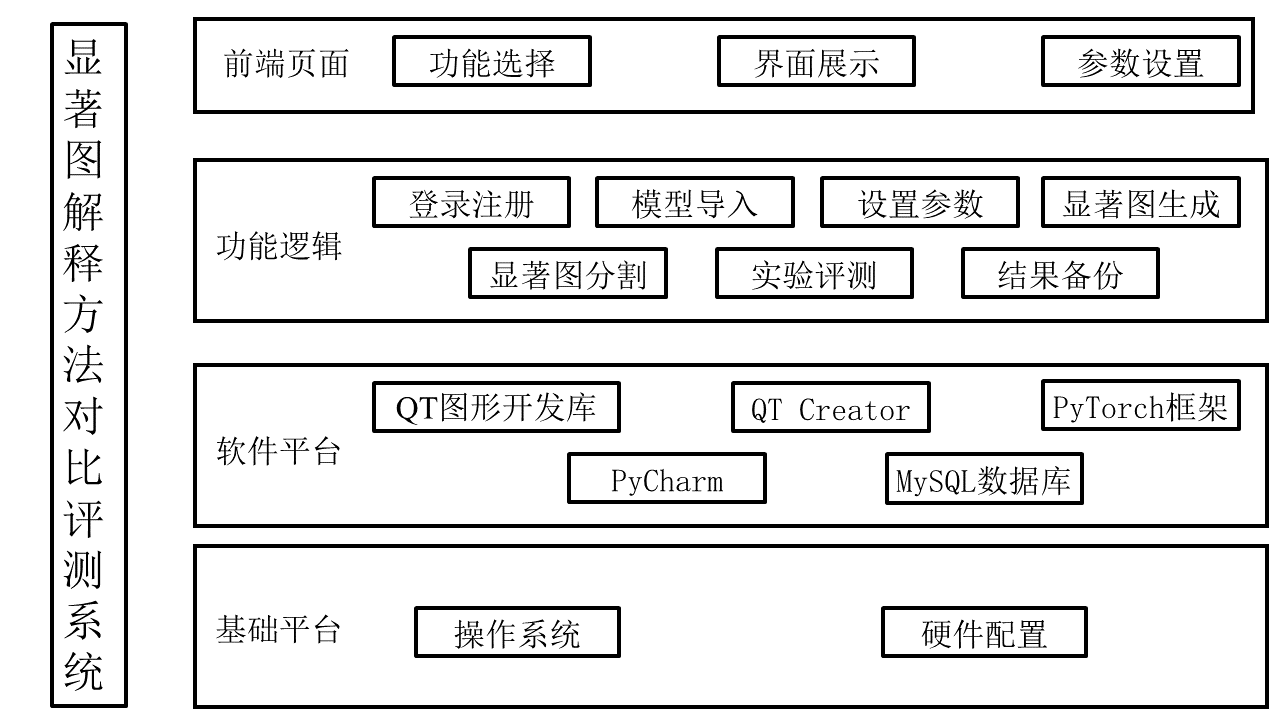
\includegraphics[width=15cm]{fig/ch5/sys.png}
	\bicaption[\xiaosi 系统架构设计图]{\wuhao 系统架构设计图}{\wuhao System architecture design diagram}
	\label{fig:sys}
\end{figure}
\subsection{模块设计}
显著图解释方法对比评测系统的主要功能可以分为用户功能模块和主要系统功能模块。用户功能模块包括用户登录注册、用户修改账号密码、模型查看和导入、显著图解释方法参数设置、用户评测数据备份。主要系统功能模块包括显著图方法生成对比、显著图方法分割对比、显著图方法实验评测。

显著图解释方法对比评测系统的模块设计图如图\ref{fig:function}所示,用户需要注册登录才能使用系统主要功能,用户的相关个人信息保存在服务端的数据库中,服务端和客户端通过http协议进行通信。

\begin{figure}[h]
	\centering 
	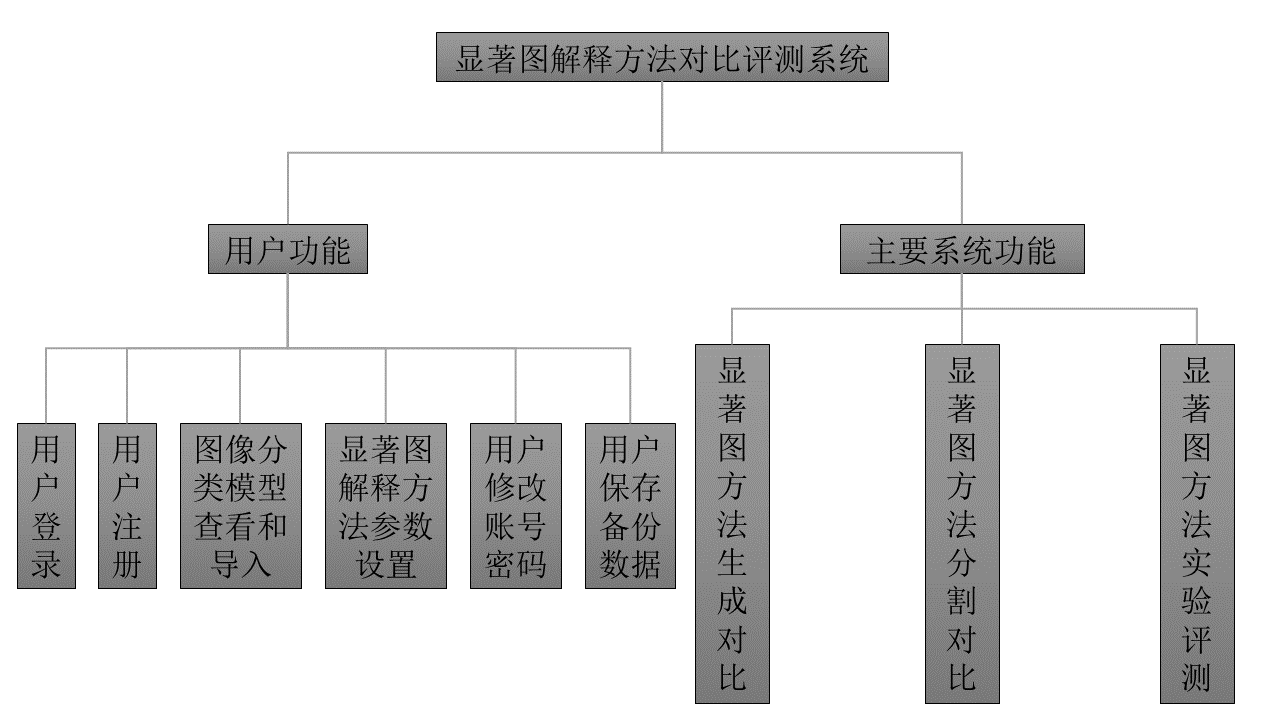
\includegraphics[width=15cm]{fig/ch5/function.png}
	\bicaption[\xiaosi 系统模块设计图]{\wuhao 系统模块设计图}{\wuhao System module design diagram}
	\label{fig:function}
\end{figure}

\subsection{功能设计}

本系统包含众多的分支功能,下面是对每个功能的详细描述:

(1)用户注册登录功能

为了记录每个用户的实验数据和显著图解释方法的配置信息,每个用户都需要注册并登录,注册后每个用户有唯一的用户账号用来在服务端数据库中保存相关实验数据。注册用户需要自定义唯一的用户名和设置登录密码,注册成功后系统会生成唯一的数字账号。后续登录功能时用户可以用用户名和数字账号进行登录。

(2)图像分类模型的查看和导入

在用户登录后,用户需要在信息设置中查看当前服务端可用的图像分类神经网络模型,用户也可自行上传合适的图像分类神经网络模型到服务端。
目前可用的图像分类模型包括:VGG16、VGG19、ResNet18、ViT。

(3)显著图解释方法的参数设置
 
在显著图解释方法的参数设置当中,用户可以看到当前可用的显著图解释方法,对于每一种显著图解释方法,用户可以自行设置参数,可以针对每一种图像分类神经网络的参数设置都会被保存到服务端,后续显著图生成选择显著图解释方法时会自动应用用户的参数设置信息,并且会根据用户选择的图像分类模型进行参数调整。目前可用的显著图解释方法包括:Grad-CAM、Grad-CAM++、Score-CAM、XGrad-CAM、RISE、Transformer Attribution、MSG-CAM。除此之外还包括本文第四章提出的增强方法,该显著图增强方法可以直接应用于上述显著图解释方法。

(4)显著图生成功能

显著图生成功能主要是方便用户在单一图片情况下直接对比不同显著图解释方法的生成效果。用户首先需要选定图像分类模型,再选择输入图片,输入图片可以从用户本地上传,选定输入图片后页面会显示用户的输入图片。然后用户需要点击按钮将该图片输入到选定的图像分类模型当中获取该图片的前5名的类别和对应概率。系统会将获取的类别和对应概率通过下拉框展示出来,用户需要选择生成显著图的类别。最后用户选择要应用的显著图解释方法,然后点击生成即可获取服务端返回的显著图。通过选择不同的显著图解释方法即可在页面上展示不同显著图解释方法的显著图,用户可以直观进行对比。

(5)显著图分割功能

显著图分割功能主要是利用显著图给出的像素优先级将原始输入图片进行分割,用户首先需要选择图像分类模型,然后选择输入图片。输入图片可以来自用户的本地上传。选定输入图片后,页面会显示用户的输入图片。接下来,用户需要点击按钮,将该图片输入到选定的图像分类模型中,以获取该图片的前5个类别及其对应概率。系统会通过下拉框展示获取的类别和对应概率,用户需要从中选择生成显著图的类别。用户需要选择要应用的显著图解释方法获取服务端返回的显著图,最后用户选择设置需要切割像素比例,此处默认将权重值排名靠前的像素进行保留,其余像素置为0。通过显著图分割可以直观对比不同显著图解释方法对物体特征的感知能力。

(6)实验测试功能

当前存在的多种实验来评测显著图解释方法,这些实验代码复杂,对于不同的显著图解释方法需要单独配置,因此该功能旨在让用户轻松进行实验。在该功能模块中用户需要选择图像分类模型,选择评测数据集,之后选择要评测的显著图解释方法,最后选择要进行的实验类型。全部选择完成后点击开始实验,客户端会将相关实验参数提交给后台服务器,后台服务器会根据实验参数自动执行脚本程序,并返回实验大致所需时间。实验完成后数据会存入用户数据库,用户之后可以查看实验结果。

(7)备份导出功能

该功能可以将用户的实验数据和相关实验参数设置保存备份。服务器将要保存的数据按规则写入纯文本文件当中,包括实验时间,实验结果,实验相关参数等,写入完成后服务端将保存备份文件传给客户端本地。

\section{系统展示}
根据本章前文的系统功能分析,本节将以图片的方式对系统主要的功能进行进一步的展示和说明。

(1)图像分类模型的查看和导入

图像分类模型的查看和导入界面如图\ref{fig:f1}所示,用户可以点击图中的导入模型按钮导入图像分类模型,此外用户还可以修改模型名称,通过输入模型编号删除个人的图像分类模型。

(2)显著图解释方法的参数设置

在图\ref{fig:f2}中展示了本文第3章提出显著图解释方法MSG-CAM的参数设置页面,用户通过选定图像分类模型,可以对该模型进行针对性的参数设置,包括选择要使用的卷积层等,每个显著图解释方法都有不同的设置页面。


(3)用户密码修改和查看功能

在图\ref{fig:f3}中展示了当前用户的数字账号和用户名等信息,用户密码默认以密文方式展示,用户需要点击查看密码按钮进行查看,同时在该页面上用户也可以修改密码。
\begin{figure}[H]
	\centering 
	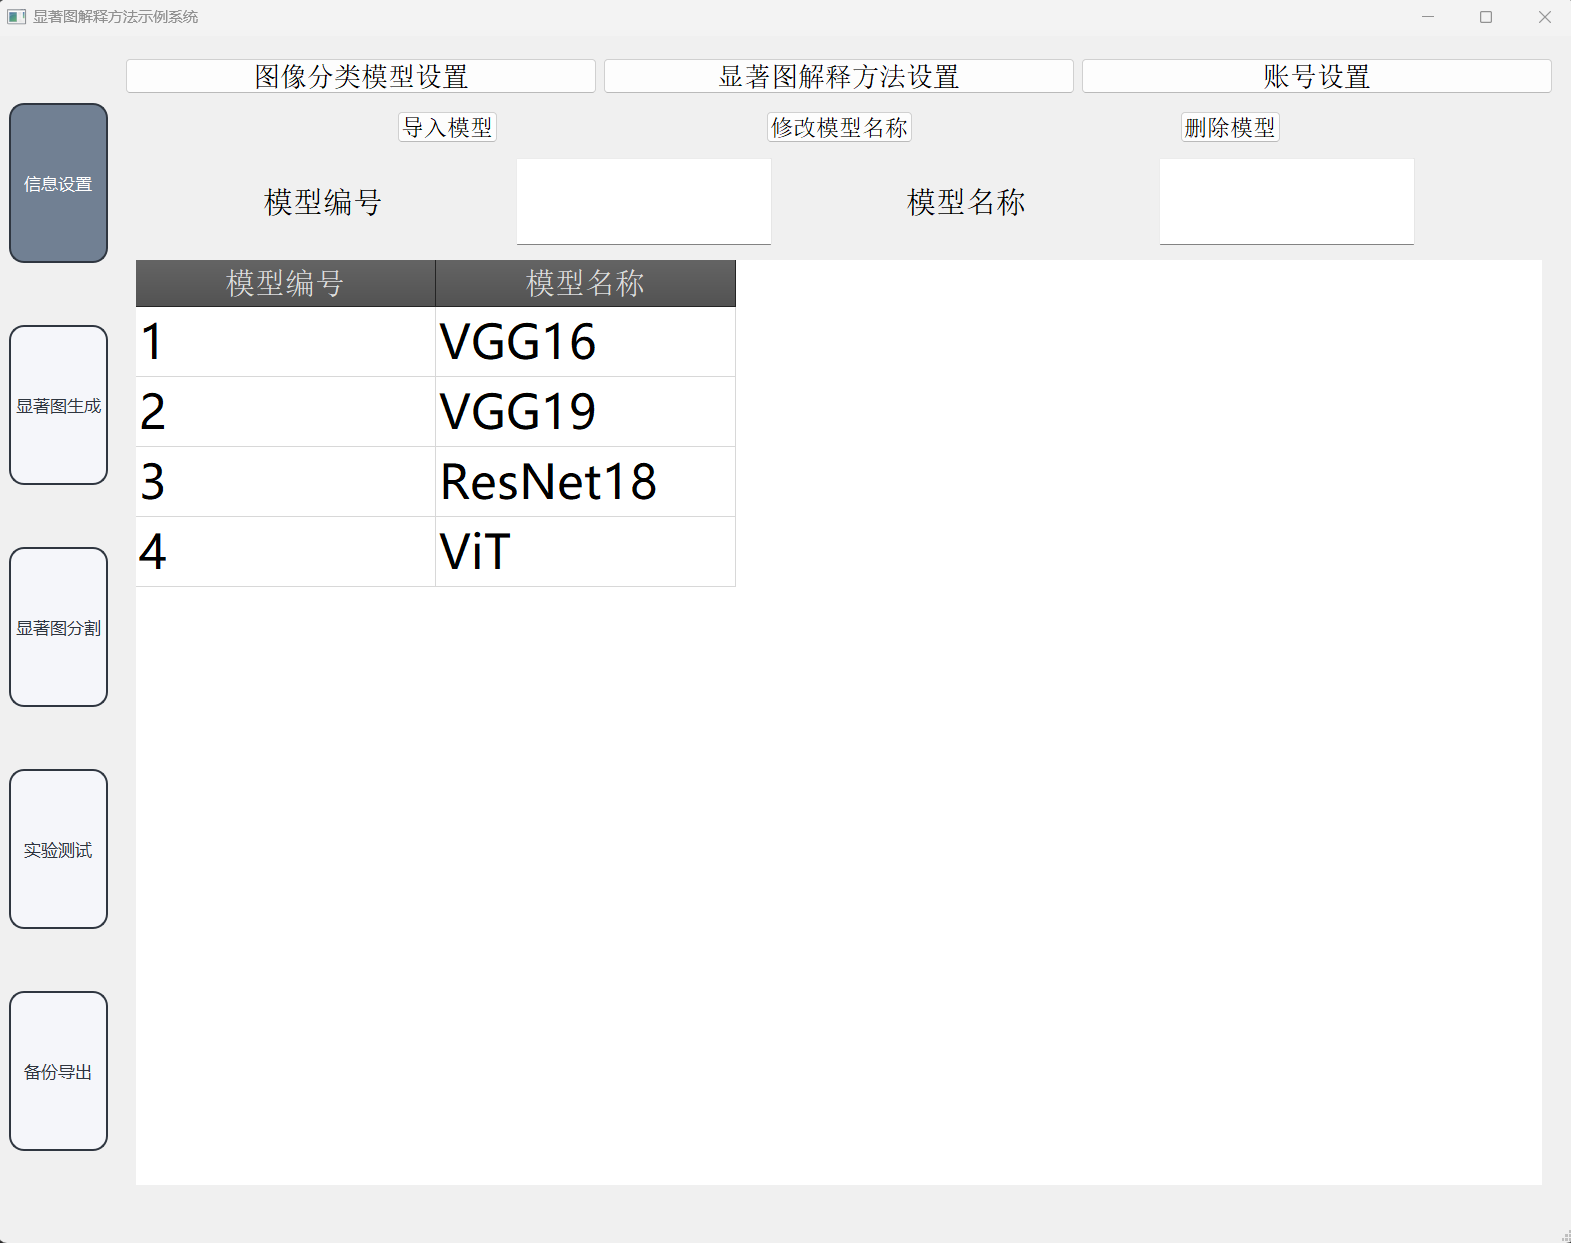
\includegraphics[width=15cm,height=9.5cm]{fig/ch5/f1.png}
	\bicaption[\xiaosi 图像分类模型的查看和导入界面图]{\wuhao 图像分类模型的查看和导入界面图}{\wuhao View and import interface for image classification models}
	\label{fig:f1}
\end{figure}

\begin{figure}[H]
	\centering 
	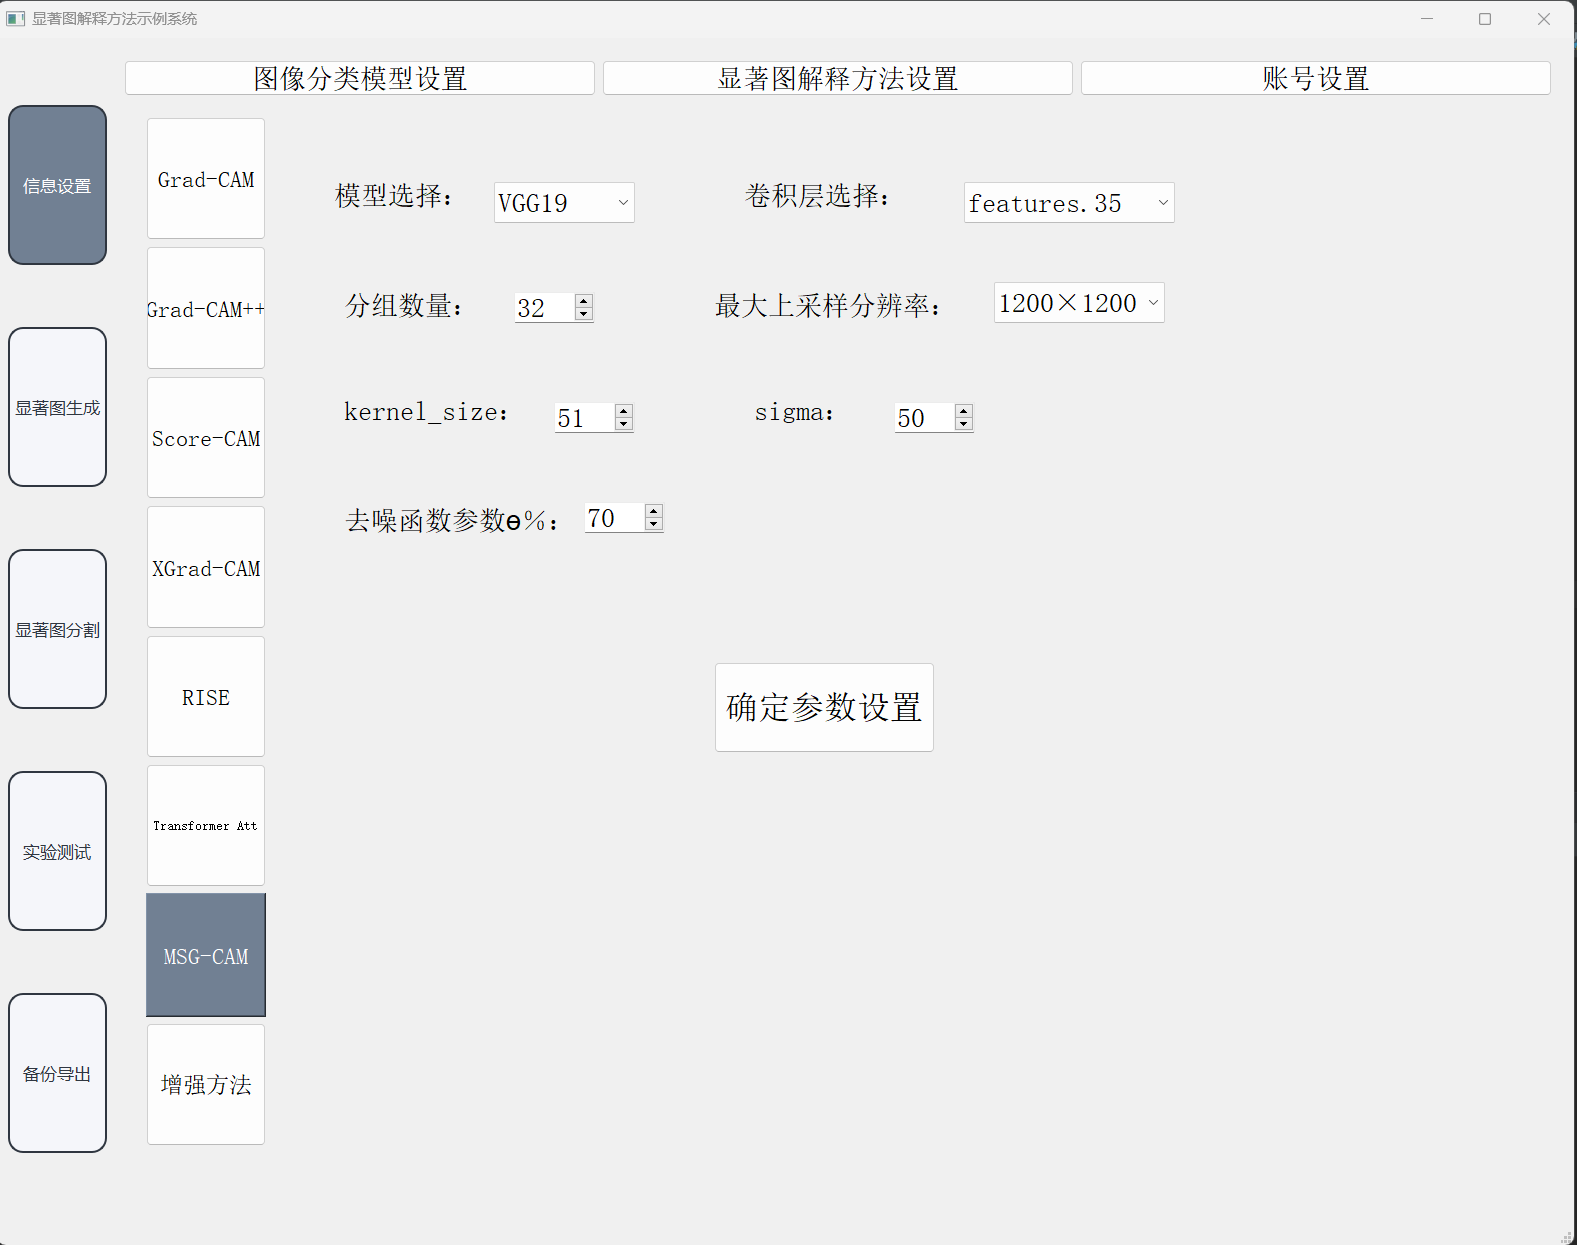
\includegraphics[width=15cm,height=9.5cm]{fig/ch5/f2.png}
	\bicaption[\xiaosi 显著图解释方法参数设置页面]{\wuhao 显著图解释方法参数设置页面}{\wuhao Saliency map method interpretation methods parameter setting page}
	\label{fig:f2}
\end{figure}

\begin{figure}[h]
	\centering 
	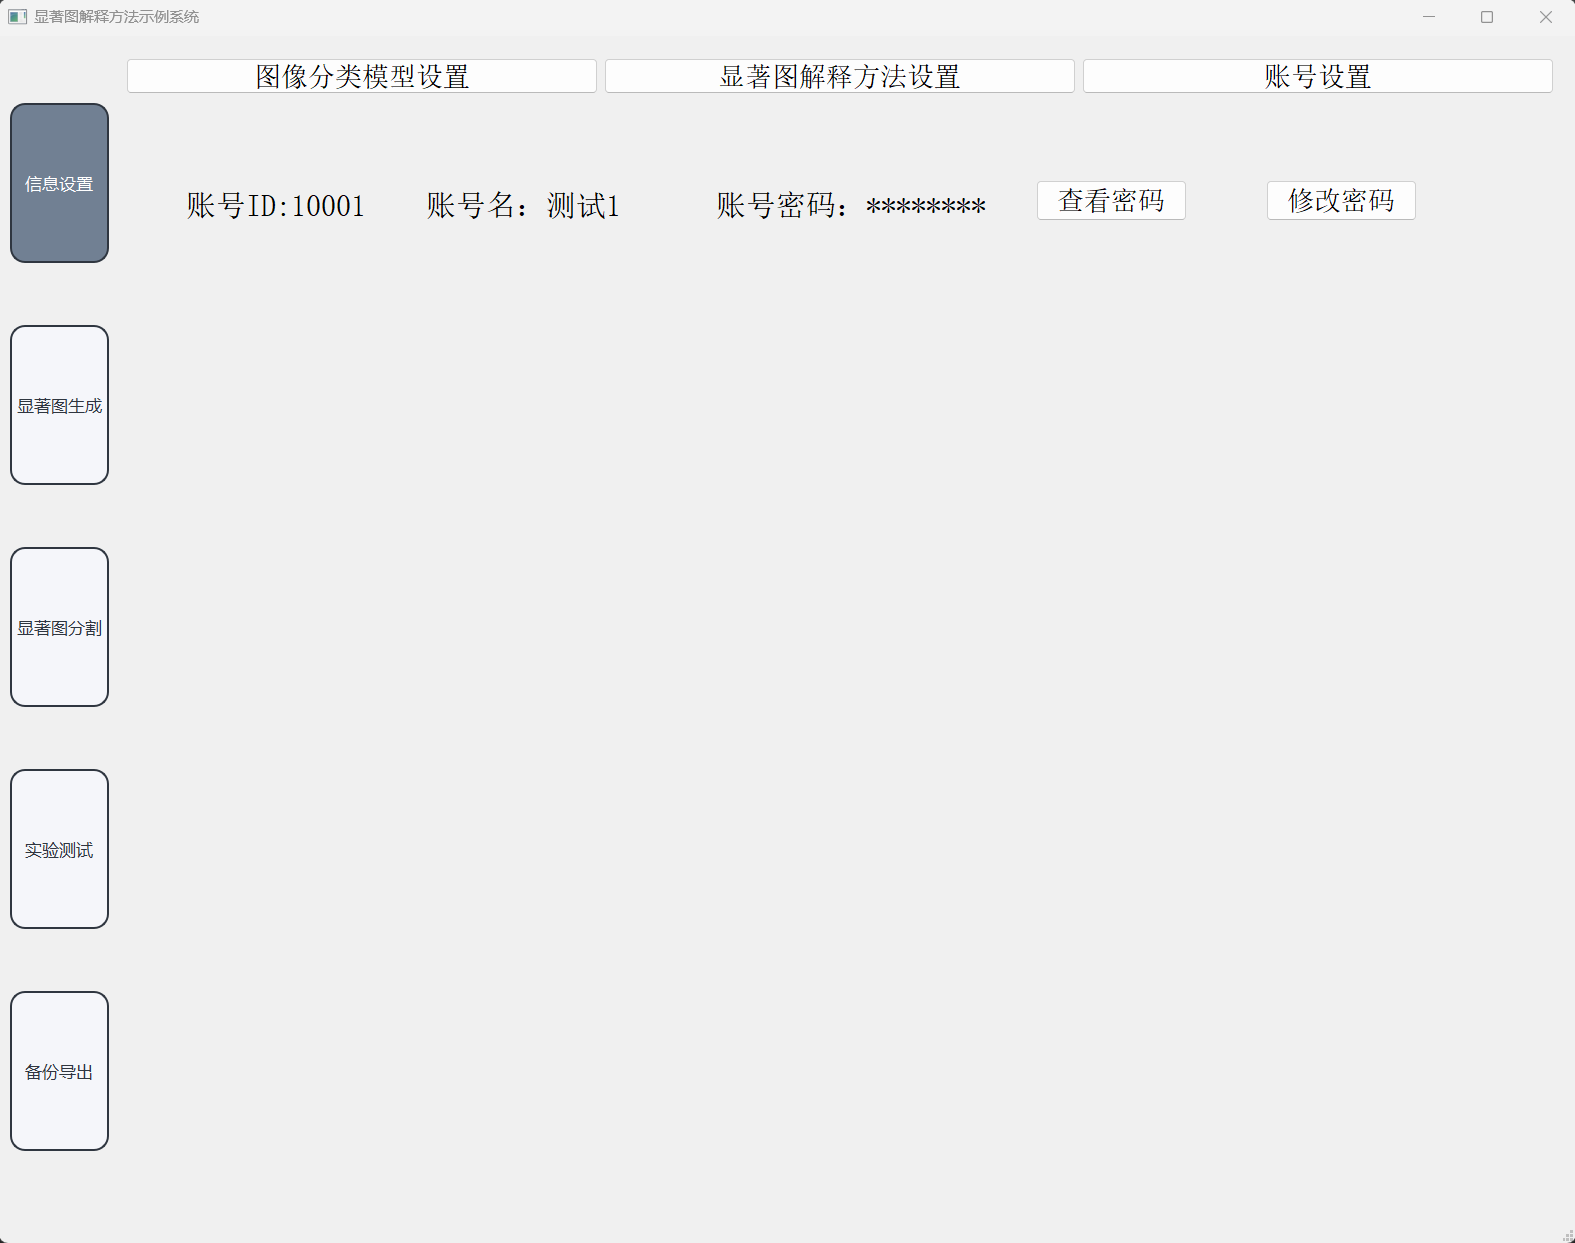
\includegraphics[width=15cm,height=9.5cm]{fig/ch5/f3.png}
	\bicaption[\xiaosi 用户密码修改和查看页面]{\wuhao 用户密码修改和查看页面}{\wuhao User password change and view page}
	\label{fig:f3}
\end{figure}
\begin{figure}[H]
	\centering 
	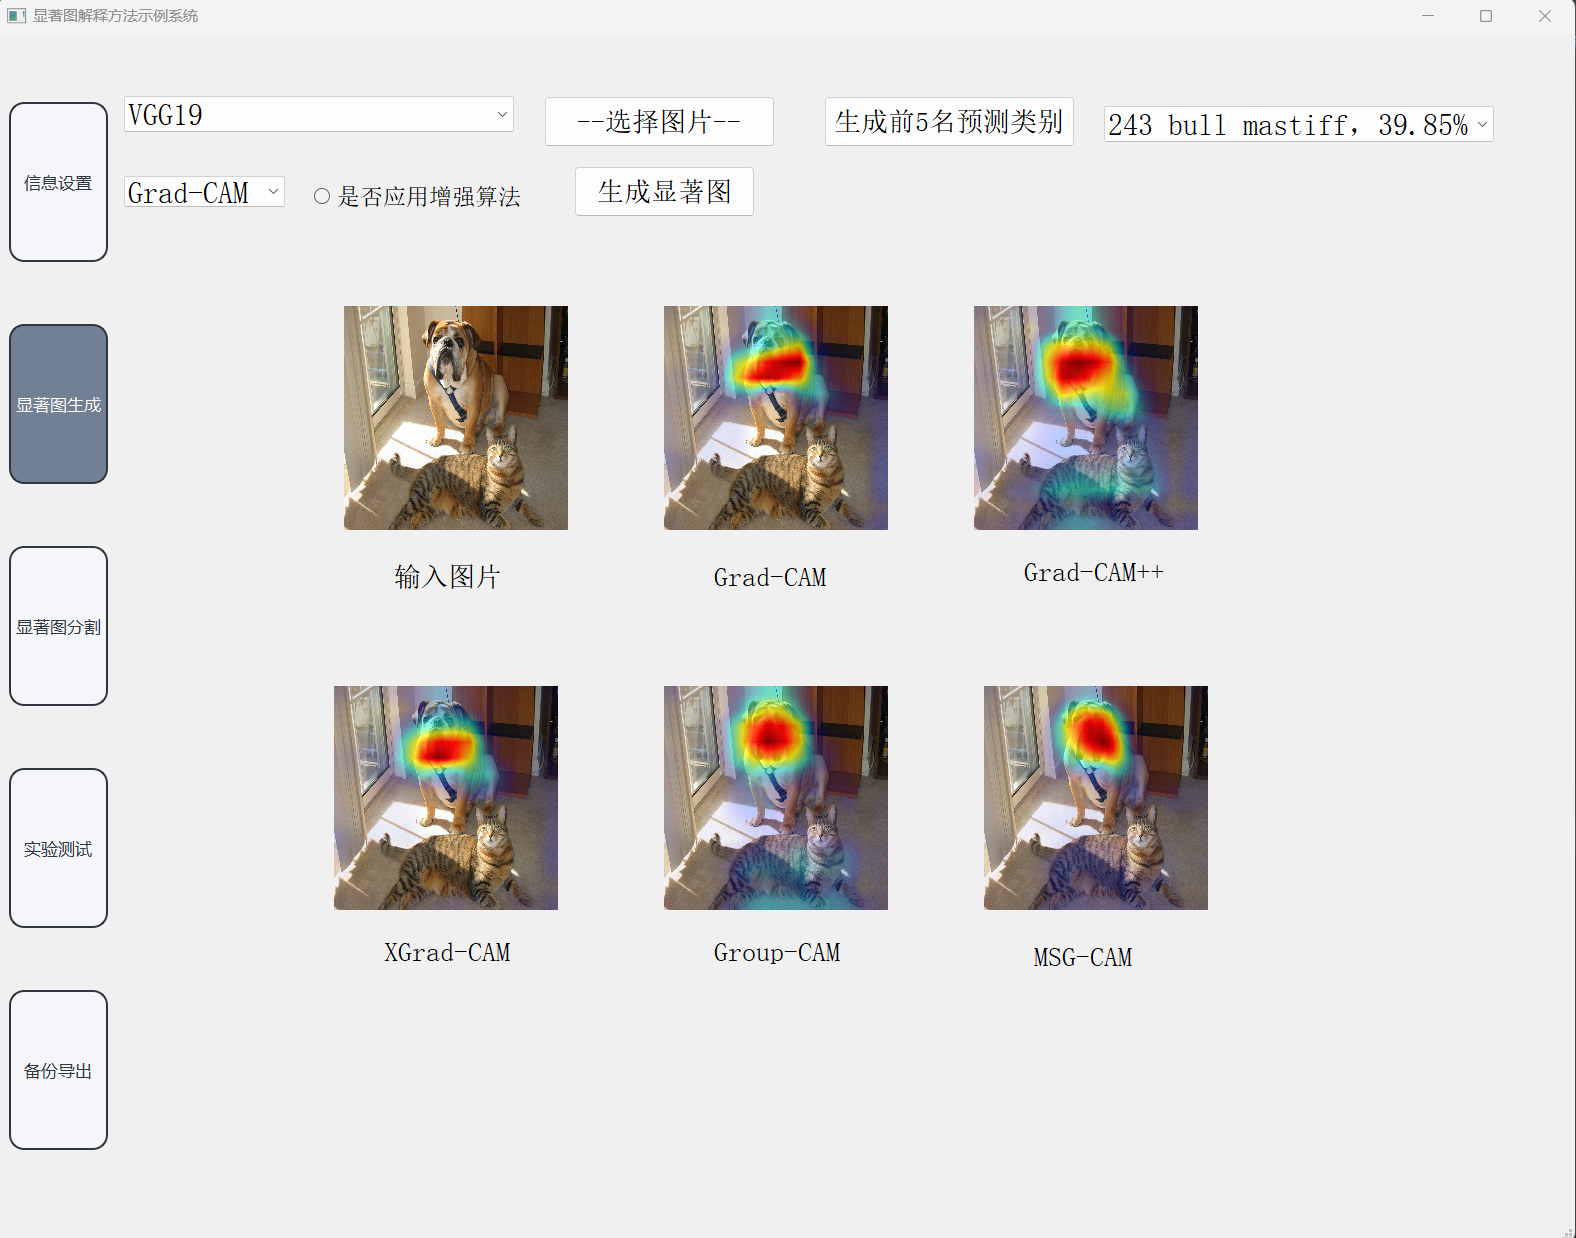
\includegraphics[width=15cm,height=9.5cm]{fig/ch5/f4.png}
	\bicaption[\xiaosi 显著图生成页面]{\wuhao 显著图生成页面}{\wuhao Saliency map generation page}
	\label{fig:f4}
\end{figure}

(4)显著图生成功能

在页面截图\ref{fig:f4}中,展示了不同显著图解释方法生成的显著图对比情况,可以看到在选择的输入图片当中,生成了前5名预测类别和相应的概率,用户还可以选择是否应用增强算法来增强该显著图解释方法生成的显著图。


(5)显著图分割功能

在图\ref{fig:f5}中展示了根据显著图进行分割情况,在该页面中用户可以设置分割使用的像素比例,选定后生成分割图界面上可以展示分割结果,用户可以直观对比不同方法分割效果,正如该图中展示的那样,在相同分割比例情况下,本文第三章提出的MSG-CAM分割效果更佳,展示了完成的物体,不相关区域更少。

\begin{figure}[h]
	\centering 
	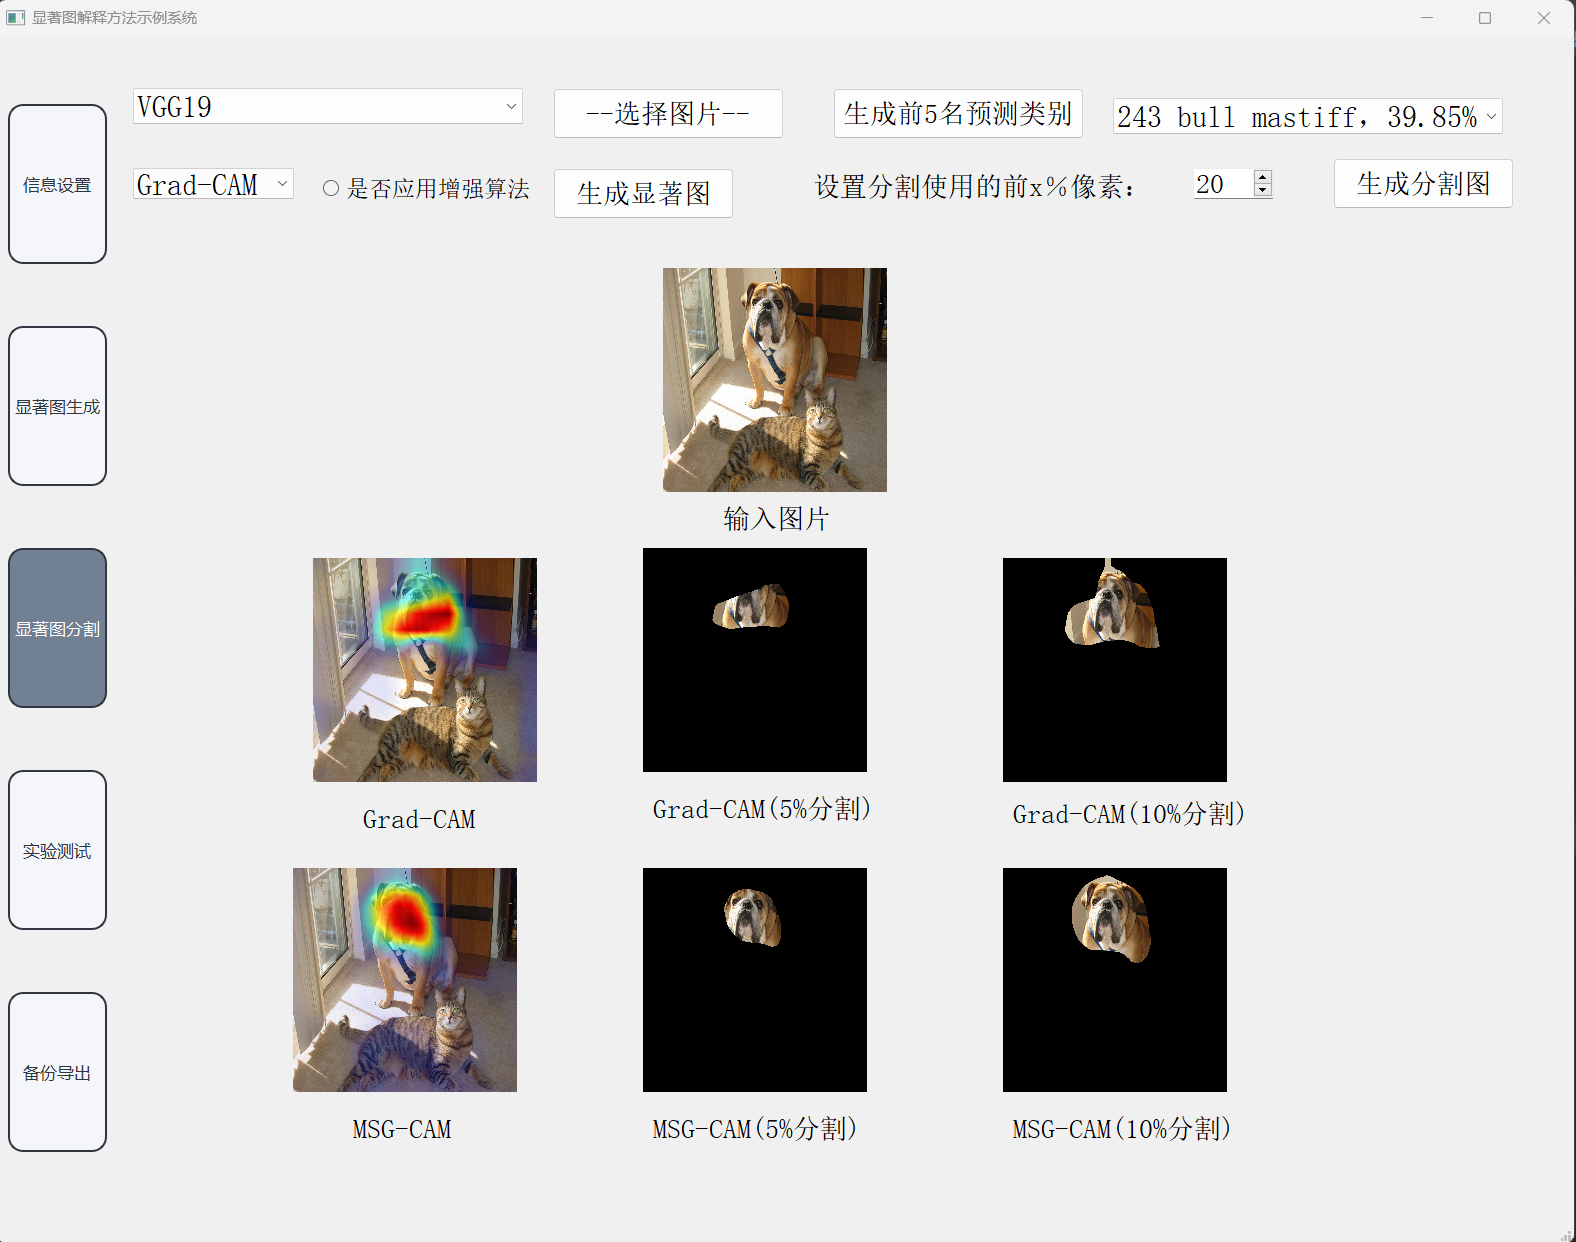
\includegraphics[width=15cm]{fig/ch5/f5.png}
	\bicaption[\xiaosi 显著图分割页面]{\wuhao 显著图分割页面}{\wuhao Saliency map segmentation page}
	\label{fig:f5}
\end{figure}

(6)实验评测功能

在图\ref{fig:f6}中展示了实验评测的页面,实验结果通过表格的方式展示在下面页面当中。

\begin{figure}[h]
	\centering 
	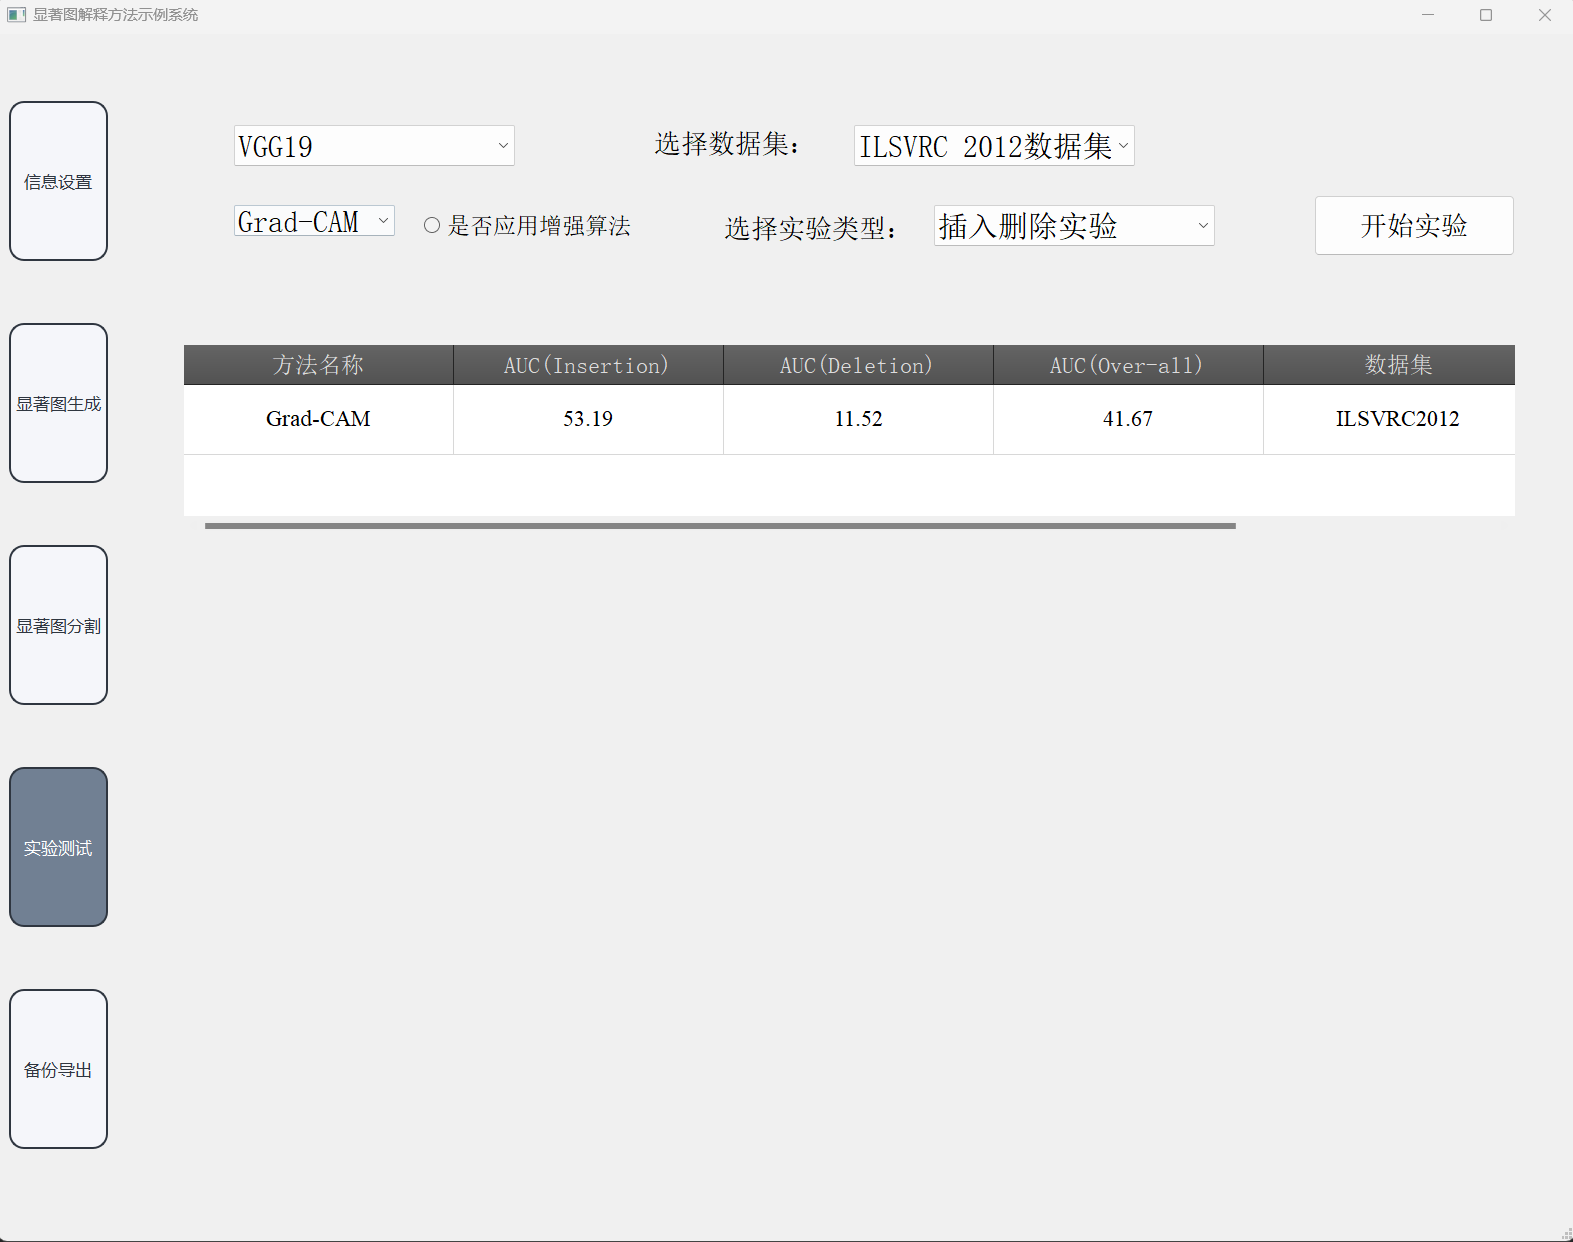
\includegraphics[width=15cm]{fig/ch5/f6.png}
	\bicaption[\xiaosi 实验评测页面]{\wuhao 实验评测页面}{\wuhao Experimental test page}
	\label{fig:f6}
\end{figure}

\section{本章小结}
本章将多种现有的显著图解释方法整合到一个统一的程序接口中,并利用软件可视化开发技术开发了一套显著图解释方法对比评测系统。该系统可以方便研究人员对当前的显著图解释方法进行对比评测,直观展现不同显著图解释方法在相同条件下的视觉差别和评测指标差异。本章通过分析需求和功能设计逐步细化系统功能,并且通过系统页面展示了原型系统的页面功能。